\documentclass[a4paper,12pt]{scrartcl}

\usepackage[utf8]{inputenc}
\usepackage[english]{babel}
\usepackage{scrpage2}
\usepackage{amsmath,amssymb}
\usepackage{verbatim}
\usepackage{color,graphicx}
% \usepackage{hyperref}

% define common URLs
\usepackage{url}
\urlstyle{tt}
\urldef{\wwwc}{\url}{http://www.w3.org}
\urldef{\owl}{\url}{http://www.w3.org/2004/OWL/}
\urldef{\owlce}{\url}{http://www.w3.org/TR/2008/WD-owl2-syntax-20081202/#Class_Expressions}
\urldef{\carc}{\url}{http://dl-learner.org/wiki/Carcinogenesis}
\urldef{\dldownload}{\url}{http://sourceforge.net/project/showfiles.php?group_id=203619}
\urldef{\mos}{\url}{http://www.co-ode.org/resources/reference/manchester_syntax/}
\urldef{\wsjavadoc}{\url}{http://dl-learner.org/javadoc/org/dllearner/server/DLLearnerWS.html}
\urldef{\wsphpexamples}{\url}{http://dl-learner.svn.sourceforge.net/viewvc/dl-learner/trunk/src/php-examples/}
\urldef{\wikiprotplugin}{\url}{http://dl-learner.org/wiki/ProtegePlugin}
\urldef{\owlapi}{\url}{http://owlapi.sourceforge.net}
\urldef{\dig}{\url}{http://dl.kr.org/dig/}

\title{DL-Learner Manual [Draft]}
\author{Jens Lehmann}

\pagestyle{scrheadings}
\automark{section}

\newcommand{\todo}[1]{\textbf{[ToDo: #1]}}

\begin{document}

\maketitle

\begin{abstract}
DL-Learner is a machine learning framework for OWL and description logics. It includes several learning algorithms and is easy to extend. DL-Learner widens the scope of Inductive Logic Programming to Descriptions Logics and the Semantic Web. This manual provides the entry point to using DL-Learner and explains its basic concepts.
\end{abstract}

\tableofcontents

\clearpage

\section{What is DL-Learner?}
\label{sec:whatis}

DL-Learner is an open source framework for (supervised) machine learning in OWL and Description Logics (from instance data). We further detail what this means:

\emph{OWL} stands for ``Web Ontology Language''. In 2004, it became the W3C\footnote{\wwwc} standard ontology language\footnote{\owl}. As such it is one of the fundamental building blocks in the Semantic Web and has been used in several scenarios on and off the web. OWL is based on \emph{description logics} (DLs), which are a family of knowledge representation languages. We refer to \cite{dlhb} for an introduction to description logics. Since OWL formally builds on description logics, we can apply DL-Learner to knowledge bases in OWL or a variety of description languages.

\emph{Machine Learning} is a subfield of Artificial Intelligence, which focuses on detecting patterns, rules, models etc.~in data. Often, this involves a training process on the input data. In \emph{Supervised} learning, this data is labelled, i.e.~we are given a number of input-output mappings. Those mappings are also called \emph{examples}. If the output is binary, then we distinguish positive and negative examples. DL-Learner as a framework is not restricted to supervised learning, but all algorithms currently build into it, are supervised.

In the most common scenario we consider, supervised learning in OWL/DLs, means that we have a background knowledge base in OWL/DLs. Additionally, we are given positive and negative examples. Each example is an individual in our knowledge base. The goal is to find an OWL \emph{class expression}\footnote{\owlce} such that all/many of the positive examples are \emph{instances} of this expression and none/few of the negative examples are instances of it. The primary purpose of learning is to find a class expression, which can classify unseen individuals (i.e.~not belonging to the examples) correctly. It is also important that the obtained class expression is easy to understand for a domain expert. We call these criteria \emph{accuracy} and \emph{readability}.

As an example, consider the problem to find out whether a chemical compound can cause cancer\footnote{see \carc{} for a more detailed description}. In this case, the background knowledge contains information about chemical compounds in general and certain compounds we are interested in. The positive examples are those compounds causing cancer, whereas the negative examples are those compounds not causing cancer. The prediction for the examples is likely to have been obtained from experiments and long-term research trials in this case. Of course, all examples have to be present in the considered background knowledge. A learning algorithm can now derive a class expression from examples and background knowledge, e.g.~this class expression in natural language could be ``chemical compounds containing a phosphorus atom''. (Of course, in practice the expression will be more complex to obtain a reasonable accuracy.) Using this class expression, we can no classify unseen chemical compounds.

\section{Getting Started}
\label{sec:start}

DL-Learner is written in Java, i.e.~it can be used on all platforms supporting Java. Currently, Java 6 or higher is required. To install the latest release, please visit the download page\footnote{\dldownload} and extract the file on your harddisk. In the top level directory, you will notice several executables. Those files ending with \verb|bat| are Windows executables, whereas the corresponding files without file extension are the Non-Windows (e.g.~Linux, Mac) executables. To test whether DL-Learner works, please run the following on the command line depending on your operating system:

\begin{verbatim}
dllearner examples/father.conf         (Non-Windows Operating System)
dllearner.bat examples/father.conf     (Windows Operating System)
\end{verbatim}

\emph{Conf files}, e.g. \verb|examples/father.conf| in this case, describe the learning problem and specify which algorithm you want to use to solve it. In the simples case they just say where to find the background knowledge to use (in the OWL file \verb|examples/father.owl| in this case) and the positive and negative examples (marked by ``+'' and ``-'', respectively). When running the above command, you should get something similar to the following:

\begin{verbatim}
DL-Learner 2008-10-13 command line interface
starting component manager ... OK (201ms)
initialising component "OWL file" ... OK (0ms)
initialising component "fast instance checker" ... OK (839ms)
initialising component "two valued definition learning problem" 
... OK (0ms)
initialising component "example driven refinement operator based 
learning algorithm" ... OK (14ms)

more accurate (83,33%) node found: http://example.com/father#male 
[q:1, he:0, children:0]
more accurate (100,00%) node found: (http://example.com/father#male 
AND EXISTS http://example.com/father#hasChild.TOP) 
[q:0, he:4, children:0]
best node (male AND EXISTS hasChild.TOP) [acc:100% h:0,962 q:0p-0n 
(REASONER), he:7 c:12]
solutions (at most 20 are shown):
1: (male AND EXISTS hasChild.TOP) (length 5, depth 3)
2: (male AND EXISTS hasChild.ALL hasChild.TOP) (length 7, depth 4)
3: (male AND EXISTS hasChild.(female OR male)) (length 7, depth 4)
Algorithm terminated succesfully.

number of retrievals: 4
retrieval reasoning time: 0ms ( 0ms per retrieval)
number of instance checks: 194 (0 multiple)
instance check reasoning time: 3ms ( 0ms per instance check)
overall reasoning time: 3ms (13,901% of overall runtime)
overall algorithm runtime: 26ms
\end{verbatim}

\todo{display accuracy of solutions}
\todo{find out why algorithm continues after finding EXISTS hasChild.TOP}

The first part of the output tells you which components are used (more on this in Section \ref{sec:components}). In the second part you see output coming from the used learning algorithm, i.e.~it can print information while running (``more accurate (83,33\%) class description found'') and the final solutions, it computed. The results are displayed in Manchester OWL Syntax\footnote{\mos}. There can be several solutions, in which case they are ordered with the most promising one in the first position. The last part of the output contains some runtime statistics.

\section{DL-Learner Architecture}

DL-Learner consists of core functionality, which provides Machine Learning algorithms for solving the learning problem, support for different knowledge base formats, an OWL library, and reasoner interfaces. There are several interfaces for accessing this functionality, a couple of tools which use the DL-Learner algorithms, and a set of convenience scripts. The general structure is illustrated in Figure \ref{fig:structure}.

\begin{figure}
 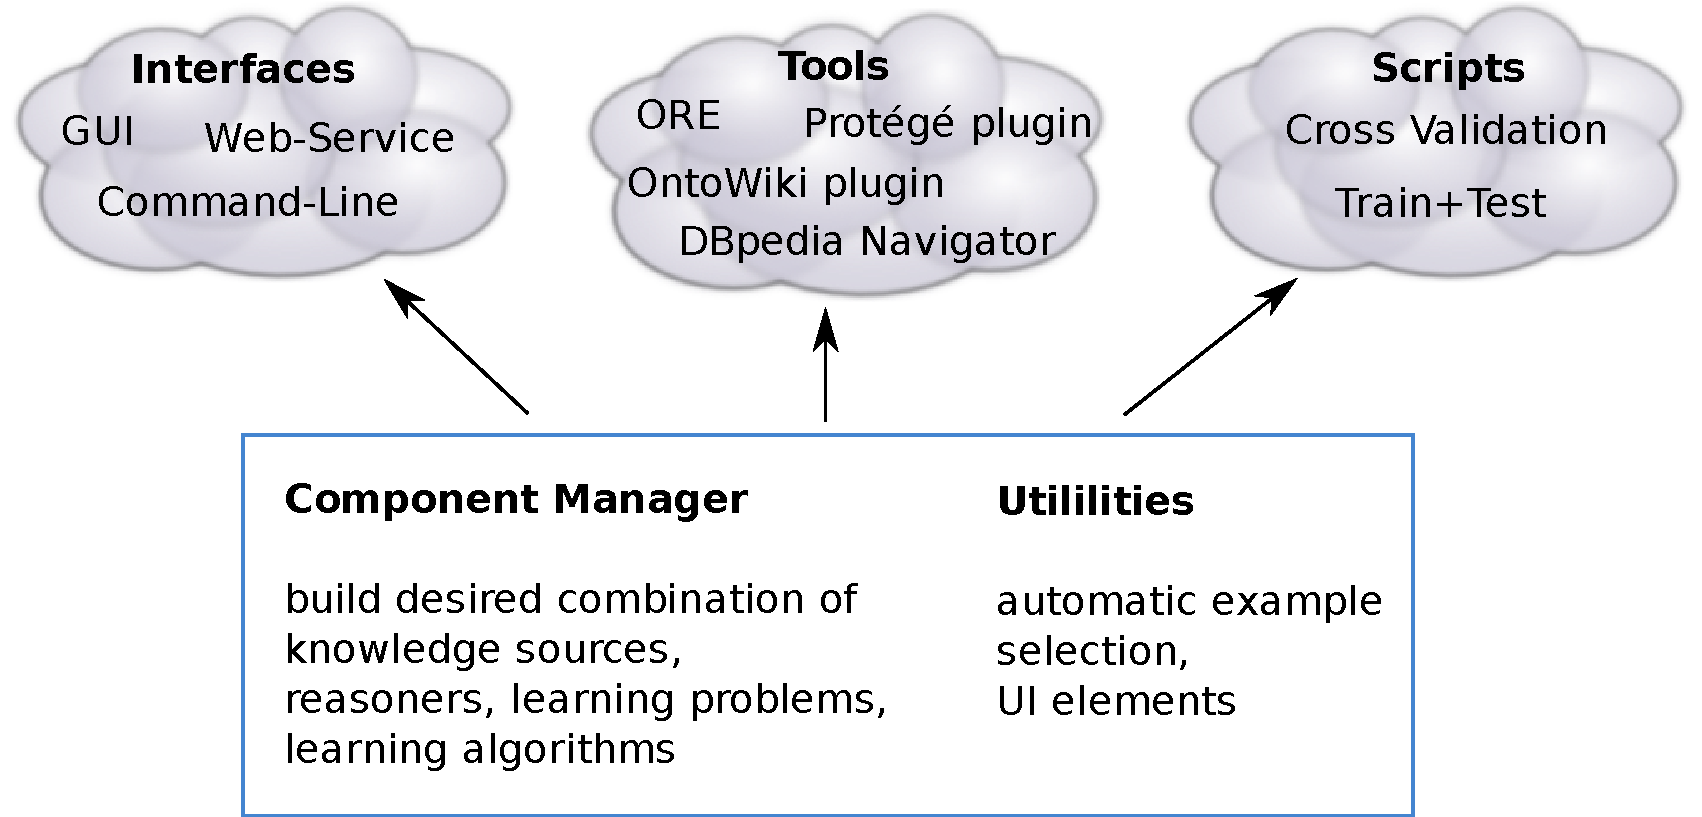
\includegraphics[width=\textwidth]{../../resources/structure_print}
 \caption{Overall structure of the DL-Learner software.}
 \label{fig:structure}
\end{figure}

To be flexible in integrating new learning algorithms, new kinds of learning problems, new knowledge bases, and new reasoner implementations, DL-Learner uses a component based model. Adding a component can be done by subclassing the appropriate class and adding the name of the new class to the “components.ini” file (more on that in Section \ref{sec:developing}).

There are four types of components (knowledge source, reasoning service, learning problem, learning algorithm). For each type, there are several implemented components and each component can have its own configuration options as illustrated in Figure \ref{fig:components}. Configuration options can be used to change parameters/settings of a component. In Section \ref{sec:components}, we describe the components in DL-Learner and their configuration options.

\begin{figure}
 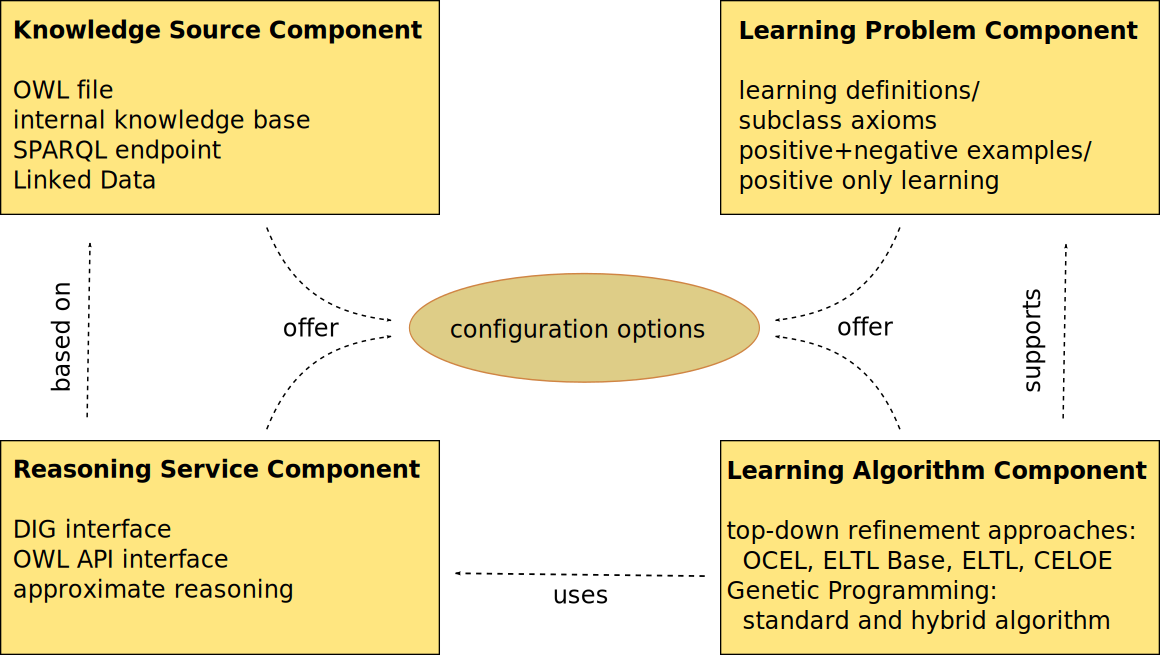
\includegraphics[width=\textwidth]{../../resources/components_print}
 \caption{The architecture of DL-Learner is based on four component types, which can each have their own configuration options. DL-Learner uses a component manager to organise all components.}
 \label{fig:components}
\end{figure}

\section{DL-Learner Components}
\label{sec:components}

In this part, we describe concrete components currently implemented in DL-Learner. Each of the subsections contains a list of components of type specified in the subsection heading. Note that this constitute a full description, i.e.~we omit some components and many configuration options. The purpose of the manual is to obtain a general understanding of the implemented components. A full list of components, which is generated automatically from the source code, can be found in \verb|doc/configOptions.txt| including the default values for all options and their usage in conf files. \todo{ConfigDocumentationGenerator seems partially broken, because it prints things like CLI usage: null = owlAPIReasoner;}

\subsection{Knowledge Sources}

Knowledge sources have a URI and can be included in conf files using \verb|import("$url");|, e.g.~\verb|import("ontology.owl")|. Depending on the file ending, DL-Learner will guess the correct type of knowledge source. If you want to overwrite this, you can use a second parameter with value \verb|OWL|, \verb|KB|, or \verb|SPARQL|, e.g.~\verb|import("ontology.owl","OWL")|.

\begin{description}
 \item[OWL File] DL-Learner supports OWL files in different formats, e.g. RDF/XML or N-Triples. If there is a standard OWL format, you want to use, but is not supported by DL-Learner please let us know.
 \item[KB File] KB files are an internal non-standardised knowledge representation format, which corresponds to description logic syntax except that the special symbols have been replaced by ASCII strings, e.g.~\verb|AND| instead of $\sqcap$. You can find several KB files in the examples folder.
 \item[SPARQL Endpoint] DL-Learner allows to use SPARQL endpoints as background knowledge source, which enables the incorporation of very large knowledge bases, e.g. DBpedia\cite{2008_dbpedia}, in DL-Learner. This works by using a set of start instances, which usually correspond to the examples in a learning problem, and then retrieving knowledge about these instances via SPARQL queries. The obtained knowledge base fragment can be converted to OWL and consumed by a reasoner later since it is now sufficiently to be processed in reasonable time. Please see \cite{2009_ijswis} for details. Some options of the SPARQL component are:
\begin{itemize}
 \item instances: Set of individuals to use for starting the knowledge fragment extraction. Example use in conf file: \begin{verbatim}sparql.instances = {"http://dbpedia.org/resource/Matt_Stone",
 "http://dbpedia.org/resource/Sarah_Silverman"};\end{verbatim}
 \item recursionDepth: Maximum distance of an extracted individual from a start individual. This influences the size of the extracted fragment and depends on the maximum property depth you want the learned class expression to have. Example use in conf file: \verb|sparql.recursionDepth = 3;|.
\end{itemize}
 Many further options allow to modify the extracted fragment on the fly or fine-tune the extraction process.
\end{description}

\subsection{Reasoner Components}

Several reasoner components are implemented, which can be interfaces to concrete reasoner implementations. To select a component in a conf file, use \verb|reasoner=$value;|, where  \verb|$value| is one of \verb|digReasoner|, \verb|fastInstanceChecker|, or \verb|owlAPIReasoner|, which are explained below.

\begin{description}
 \item[OWL API] The OWL API\footnote{\owlapi} reasoner interface can be used in conjunction with the Pellet and FaCT++ reasoners. The only option allows to switch between both:
 \begin{itemize}
  \item reasonerType: Selects the desired reasoner. By default, Pellet is used. Usage: \verb|owlAPIReasoner.reasonerType = fact;|. Note that FaCT++ is written in C++ and we currently ship the 32 bit version of the JNI layer. This may change to 64 bit in the future.
 \end{itemize}
 \item[DIG] DIG 1.1\footnote{\dig} is an interface to description logic reasoners and supported by a large variety of reasoners including Pellet, FaCT++, KAON2, and Racer Pro. The major drawback is that the current version DIG 1.1 is not aligned with the OWL specification and therefore lacks several features, which are crucial to the more recent learning algorithms in DL-Learner. If you still want to use the DIG interface, you have to download a DIG capable reasoner and start the DIG server there. DL-Learner communicates with the reasoner using the XML based protocol over HTTP.
 \item[Fast Instance Checker] Instance checks, i.e.~testing whether an individual is instance of a class, is the major reasoner task in many learning algorithms. This reasoner is a self-developed for the DL-Learner project. It remedies some problems related to Machine Learning and the Open World Assumption in OWL and therefore is not correct w.r.t.~OWL semantics. (See \cite{cheng00} Section 4 for an explanation.) Furthermore, it provides an improved performance for instance checks by precomputing some inferences. The fast instance checker is build on top of Pellet and the default reasoner component in DL-Learner.
\end{description}

\subsection{Learning Problems}

In the introduction Sections \ref{sec:whatis} and \ref{sec:start}, we described a specific learning problem where positive and negative examples are given. In practice different variations of similar problems occur. You can switch between the different problems using \verb|problem=$value;|, where \verb|$value| is one of \verb|posNegDefinitionLP|, \verb|posOnlyDefinitionLP|, \verb|classLearning|.

\begin{description}
 \item[Positive and Negative Examples] Let the name of the background ontology be $\mathcal{O}$. The goal in this learning problem is to find an OWL class expression $C$ such that all/many positive examples are instances of $C$ w.r.t.~$\mathcal{O}$ and none/few negative examples are instances of $C$ w.r.t.~$\mathcal{O}$. As explained previously, $C$ should be learned such that it generalises to unseen individuals and is readable. The important configuration options of this component are obviously the positive and negative examples, which are often indicated with \verb|+| and \verb|-| signs in conf files as an optional shortcut to using e.g.~\verb|posNegDefinitionLP.positiveExamples = {...}|.
 \item[Positive Examples] This learning problem is similar to the one before, but without negative examples. In this case, it is desirable to find a class expression which closely fits the positive examples while still generalising sufficiently well. For instance, you usually do not want to have \verb|owl:Thing| as a solution for this problem, but neither do you want to have an enumeration of individuals.
 \item[Class Learning] In class learning, you are given an existing class $A$ within your ontology $\mathcal{O}$ and want to describe it. It is similar to the previous problem in that you can use the instances of the class as positive examples. However, there are some differences, e.g.~you do not want to have $A$ itself as a solution of the problem, and since this is an ontology engineering task, the focus on short and readable class expressions is stronger than for the two problems mentioned before. \todo{This is under construction, but will be implemented soon.}
\end{description}

\subsection{Learning Algorithms}

The implemented algorithms vary from very simple (and usually inappropriate) algorithms to sophisticated ones. You can switch between the different algorithms using \verb|algorithm=$value;|, where \verb|$value| is one of \verb|bruteForce|, \verb|random|, \verb|gp|, \verb|refinement|, \verb|refexamples|, and \verb|celoe|. \todo{Rename refexamples to refinement2.}

\begin{description}
 \item[Brute Force]: This algorithm tests all class expressions up to a specified length, which you can set using e.g.~\verb|bruteForce.maxlength = 7|.
 \item[Random Guesser]: This algorithm randomly generates class expressions. To do this it creates trees, which can be mapped to class expressions. Its main parameter is the number of created trees, which you can set using e.g.~\verb|random.numberOfTrees = 5|.
 \item[Genetic Programming (GP)]: GP is a well-known general problem solution method, which can be adapted to class expression learning. The adaption is straightforward. In DL-Learner, however, an additional genetic refinement operator was implemented, which has shown to improve GP performance\cite{hybrid_gp}. Some options are:
 \begin{itemize}
  \item number of individuals: The individual count is the size of each generation in a GP algorithm. It is one of the most crucial parameters. Setting it to a higher value usually means investing more computational resource for increasing the likelihood that a solution will be found. Usage: \verb|gp.numberOfIndividuals = 100|
  \item refinement probability: This is used to specify how likely the usage of the genetic refinement operator should be, e.g.~\verb|gp.refinementProbability = 0.6| means that it will be selected 60\% of the time.
 \end{itemize}
 The GP algorithm has 15 more options documented in \verb|doc/configOptions.txt|.
 \item[Refinement] This is a top down refinement operator approach, which is described in \cite{alc_learning_algorithm}. Some options include:
 \begin{itemize}
  \item target language: The standard target language of this algorithm is $\mathcal{ALCN(D)}$. However, you can specify the target language in more detail, i.e.~you can exclude the $\forall$ constructor by using \verb|refinement.useAllConstructor = true;|. Similar options exist for $\exists$, $\not$, cardinality restrictions, and boolean datatypes.
  \item maximum execution time: If there is no perfect solution of a given problem, the algorithm can potentially run forever (in practice it will run out of memory). It is therefore often interesting to limit the execution time. You can use e.g.~\verb|refinement.maxExecutionTimeInSeconds = 100| to say that the algorithm should run for at most 100 seconds. Often, it will run slightly longer than the maximum executiontime since it waits until the next internal loop of the algorithm to stop gracefully.
 \end{itemize}
  The algorithm supports a range of further options. For instance, one can specify which classes and properties must not occur in resulting class expressions.
 \item[Refinement II] The previous algorithm has been extended to make more sophisticated use of background knowledge and therefore run more efficiently on many problems. It also supports double datatypes and hasValue restrictions (which again can be turned on or off as desired). It also includes explicit noise handling through the \verb|noisePercentage| option. This is currently the default and recommend algorithm for learning from positive and negative examples. More than 30 options can be set to control its behaviour. However, apart from the target language the most important setting is noise, which should be optimised for the given problem. \todo{say more about it?, include option descriptions?, rename noise to minAccuracy which describes it better}
 \item[Class Expression Learning for Ontology Engineering (CELOE)] \todo{This algorithm is under construction.}
\end{description}

Please note that while components are interchangeable, it is not possibly to arbitrarily combine them. For instance, the newer learning algorithms do not work with the DIG interface, since it does not provide the necessary inference tasks. Furthermore, a learning algorithm can specify which learning problems it can solve, i.e.~we do not require a learning algorithm to be able to solve each learning problem. In later versions of this manual, we may include a compatibility matrix. In the meantime, you can easily verify whether a combination works by testing it in a conf file.

\section{DL-Learner Interfaces}

One interface you have already used in Section \ref{sec:start} is the command line. There are two executables, which can be used for starting DL-Learner on the commandline: \verb|dl-learner| and \verb|quickstart|. The first one takes a conf file as argument, whereas the latter one lists all conf files in the examples folder and allows you to select one of those.

\begin{figure}
 \centering
 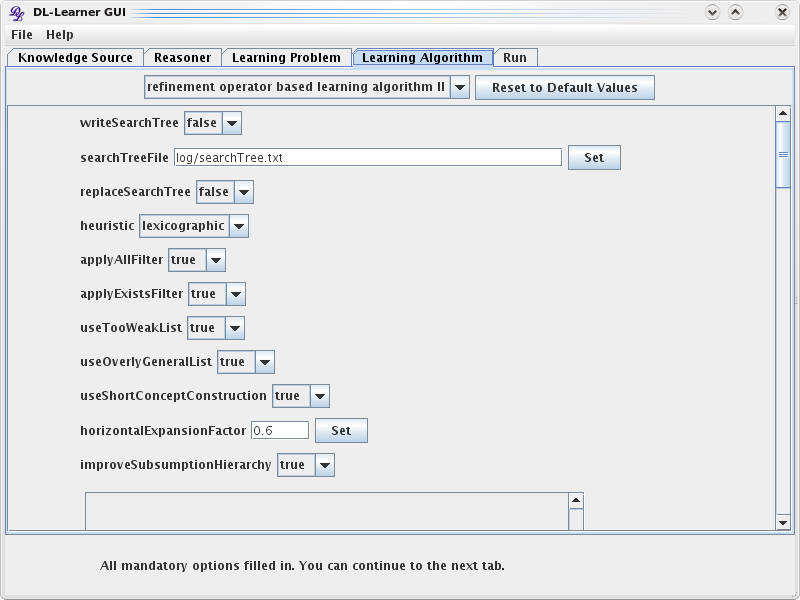
\includegraphics[width=.8\textwidth]{../../resources/screenshots/gui_algorithm}
 \caption{GUI screenshot showing the learning algorithm tab. The UI allows you to set different options and then proceed to the next tab and execute the algorithm.}
 \label{fig:gui}
\end{figure}

Apart from the command line, there is also a prototypical graphical interface. You can use \verb|gui| (or \verb|gui.bat|) to start it. You can optionally pass it a conf file as argument. The main GUI window has four tabs corresponding to the four different types of components and a run tab to execute the learning algorithm. Using the GUI, you can assemble the desired combination of components and options. The \verb|File| menu allows you to load a conf file or save the current configuration to a conf file. The GUI implementation is currently prototypical, so please report any bugs or feature requests you have (see Section \ref{sec:contact}). Since the GUI uses the component manager, it will automatically evolve when new components and options are added.

A third interface through which DL-Learner can be accessed programmatically is a web service. You can execute \verb|ws| (or \verb|ws.bat|) to start the web service. It is based on the Java API for XML Web Services (JAX-WS), which is included in Java 6 or higher. Executing the command will start a web server on port 8181 of your local machine. The WSDL can be accessed via \url{http://localhost:8181/services?wsdl}. You can use a WSDL viewer to see the supported operation 
or view the JavaDoc of the corresponding Java file\footnote{viewable online at \wsjavadoc}. 
Some examples for calling the web service from PHP can be found in the DL-Learner subversion 
repository\footnote{in the directory src/php-examples/:\\ \wsphpexamples}.
\todo{Javadoc of web service needs to be improved (almost undocumented)}

Another means to access DL-Learner, in particular for ontology engineering, is to use the OntoWiki and Protégé plugins. The OntoWiki plugin is not officially released yet, but can be used in the SVN version of OntoWiki. The Protégé 4 plugin can be installed either by downloading it from the DL-Learner download page or directly within Protégé 4 by clicking on ``File'', ``Preferences'', ``Plugins'', ``Check for Downloads'' now and selecting the DL-Learner plugin. For more information and a screencast see the Protégé plugin wiki page \footnote{\wikiprotplugin}.

\section{Extending DL-Learner}
\label{sec:developing}

DL-Learner is open source and component based. If you want to develop a specific part or extension of a class expression learning algorithm for OWL, then you are invited to use DL-Learner as a base. This allows you to focus on the part you want to implement while being able to use DL-Learner as a library and access it through one of the interfaces. In a first step, you have to decide which type of component you want to create. To implement a concrete component, you have to subclass one of the following classes and implement their abstract methods:

\begin{itemize}
 \item org.dllearner.core.KnowledgeSource
 \item org.dllearner.core.ReasonerComponent
 \item org.dllearner.core.LearningProblem
 \item org.dllearner.core.LearningAlgorithm
\end{itemize}

You then have to add your component to \verb|lib/components.ini| such that it is registered in the component manager when DL-Learner starts up. If you want to use configuration options in your component, you need to create a static method as follows:

\begin{verbatim}
public static Collection<ConfigOption<?>> createConfigOptions() {
  List<ConfigOption<?>> options = new LinkedList<ConfigOption<?>>();
  options.add(new IntegerConfigOption("maxDepth", 
    "maximum depth of generated concepts/trees", 5));
  return options;
}
\end{verbatim}

This creates an option with name \verb|maxDepth|, the given description, and a default value of 5. To add further options, simply add more of them to the collection. Running \verb|org.dllearner.scripts.ConfigJavaGenerator| generates a file for you in package \verb|org.dllearner.configurators| to access the options of your component programmatically if desired. Currently, the following configuration option types exist (new ones can be implemented if necessary):

\begin{itemize}
 \item boolean, e.g. \verb|useCache|
 \item string (a set of allowed strings can be specified), e.g. \verb|cacheDir|
 \item URL, e.g. \verb|reasonerURL|
 \item int (min and max value can be specifified), e.g. \verb|maxDepth|
 \item double (min and max value can be specifified), e.g. \verb|noisePercentage|
 \item set of strings, e.g. \verb|positiveExamples|
 \item list of string tuples, e.g. \verb|replaceObject|
\end{itemize}

Although, we loose the ability to use arbitrary argument types as options in components, this gives us the possibility to build very flexible user interfaces. Whenever, a new component or a new configuration option for a component is added, the current user interfaces (GUI, web service, commandline) will automatically support it without any or only minimal code changes.

This quick introduction only serves as an entry point to get you started. For more detailed questions about how to extend DL-Learner, please drop us a message in the DL-Learner mailing list.

\section{General Information}
\label{sec:general}
\label{sec:contact}

\begin{itemize}
 \item Homepage: \url{http://dl-learner.org}
 \item Sourceforge.net project page: \url{http://sourceforge.net/projects/dl-learner/}
 \item Tracker (bugs, features): \url{http://sourceforge.net/tracker/?group_id=203619}
 \item Mailing Lists: \url{http://sourceforge.net/mail/?group_id=203619}
 \item Contact: lehmann@informatik.uni-leipzig.de (please use the mailing list if possible)
 \item Latest Release: \url{http://sourceforge.net/project/showfiles.php?group_id=203619}
\end{itemize}

\bibliographystyle{apalike}
\bibliography{bibliography}

\end{document}

